The equation of a plane is given as
\begin{align}\label{eq:solutions/line_plane/83e1}
    \vec{n}^T\vec{x} = c
\end{align}
where $\vec{n}$ = normal vector to the plane

Let $\vec{O} = \myvec{0\\0\\0}$ be the origin and $\vec{P} = \myvec{x_1\\y_1\\z_1}$ be the foot of the perpendicular drawn from the origin to the plane.

The position vector from $\vec{O}$ to $\vec{P}$ is $(\vec{P} - \vec{O})$

Since $(\vec{P} - \vec{O})$ is perpendicular to the plane, it is parallel to the normal of the plane $\vec{n}$. So,
\begin{align}
    \vec{P} - \vec{O} = k\vec{n}\\
    \vec{P} = k\vec{n} + \vec{O}
\end{align}
where $k$ is any scalar quantity.

Since $\vec{O}$ is a null vector,
\begin{align}\label{eq:solutions/line_plane/83e2}
    \implies\vec{P} = k\vec{n}
\end{align}
Since $\vec{P}$ lies on the given plane, it must satisfy the equation of the plane. Therefore,
\begin{align}
    \vec{n}^T\vec{P} = c\\
    \implies\vec{n}^T(k\vec{n}) = c\\
    \label{eq:solutions/line_plane/83e3}\implies k\vec{n}^T\vec{n} = c
\end{align}
a)$\myvec{2&3&4}\vec{x} = 12$

Comparing with \eqref{eq:solutions/line_plane/83e1}, we get $\vec{n}^T = \myvec{2&3&4}$ and  $c=12$. Using this in \eqref{eq:solutions/line_plane/83e3}
\begin{align}
	k\myvec{2&3&4}\myvec{2\\3\\4} = 12\\
	\implies 29k = 12\\
	\implies k = \frac{12}{29}
\end{align}
\begin{align}
	\vec{P} = k\vec{n}
	\implies\vec{P} = \frac{12}{29}\myvec{2\\3\\4}\\
	\implies\vec{P}= \myvec{\dfrac{24}{29}\\\dfrac{36}{29}\\\dfrac{48}{29}}
\end{align}
b)$\myvec{3&4&-6}\vec{x} = 0$

Comparing with \eqref{eq:solutions/line_plane/83e1}, we get $\vec{n}^T = \myvec{3&4&-6}$ and  $c=0$. Using this in \eqref{eq:solutions/line_plane/83e3}
\begin{align}
	k\myvec{3&4&-6}\myvec{3\\4\\-6} = 0\\
	\implies -11k = 0\\
	\implies k = 0
\end{align}
\begin{align}
	\vec{P} = k\vec{n}
	\implies\vec{P} = 0\myvec{2\\3\\4}\\
	\implies\vec{P}= \myvec{0\\0\\0}
\end{align}
This shows that the plane $\myvec{3&4&-6}\vec{x} = 0$ passes through the origin.\\

c) $\myvec{1&1&1}\vec{x} = 1$\\

Comparing with \eqref{eq:solutions/line_plane/83e1}, we get $\vec{n}^T = \myvec{1&1&1}$ and  $c=1$. Using this in \eqref{eq:solutions/line_plane/83e3}
\begin{align}
	k\myvec{1&1&1}\myvec{1\\1\\1} = 1\\
	\implies 3k = 1\\
	\implies k = \frac{1}{3}
\end{align}
\begin{align}
	\vec{P} = k\vec{n}
	\implies\vec{P} = \frac{1}{3}\myvec{1\\1\\1}\\
	\implies\vec{P}= \myvec{\frac{1}{3}\\\frac{1}{3}\\\frac{1}{3}}
\end{align}
d) $\myvec{0&5&0}\vec{x} = -8$
\begin{align}
    \nonumber\implies\myvec{0&-5&0}\vec{x} = 8
\end{align}
Comparing with \eqref{eq:solutions/line_plane/83e1}, we get $\vec{n}^T = \myvec{0&-5&0}$ and  $c=8$. Using this in \eqref{eq:solutions/line_plane/83e3}
\begin{align}
	k\myvec{0&-5&0}\myvec{0\\-5\\0} = 8\\
	\implies 25k = 8\\
	\implies k = \frac{8}{25}
\end{align}
\begin{align}
	\vec{P} = k\vec{n}
	\implies\vec{P} = \frac{8}{25}\myvec{0\\-5\\0}\\
	\implies\vec{P}= \myvec{0\\\dfrac{-8}{5}\\0}
\end{align}
The Figures for the planes are shown in order:
\ref{myfig:solutions/line_plane/83}
%\renewcommand{\thefigure}{a}
\begin{figure}[h!]
    \centering
    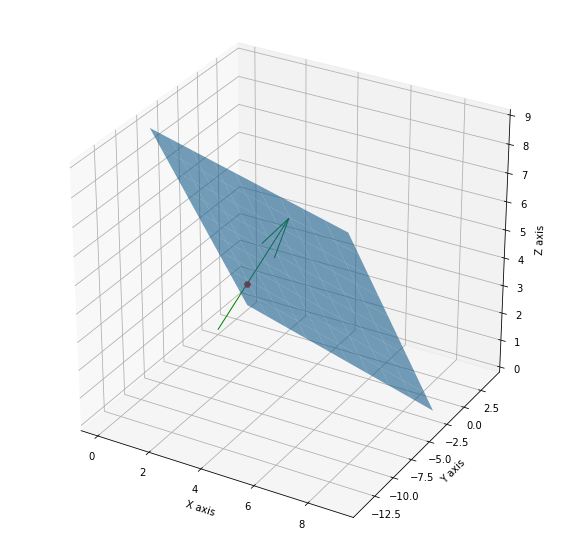
\includegraphics[width=\columnwidth]{./solutions/line_plane/83/plane1.png}
    \caption{Perpendicular drawn from origin to the plane $\myvec{2&3&4}\vec{x} = 12$}
    \label{myfig:solutions/line_plane/83}
\end{figure}
See Fig. \ref{myfig:solutions/line_plane/83}.
%\renewcommand{\thefigure}{b}
%\begin{figure}[h!]
%    \centering
%    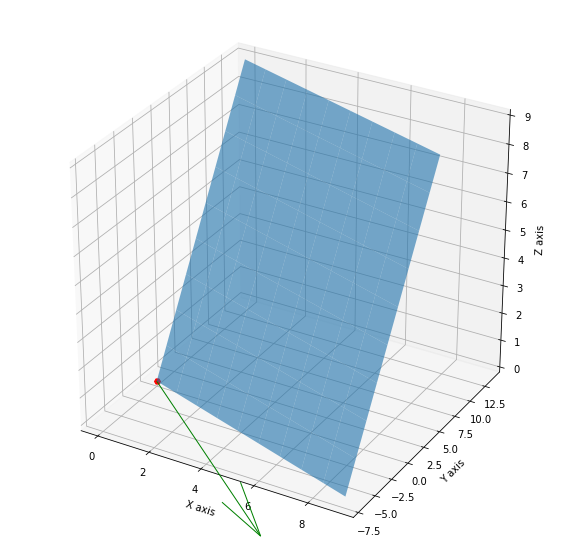
\includegraphics[width=\columnwidth]{plane2.png}
%    \caption{Perpendicular drawn from origin to the plane $\myvec{3&4&-6}\vec{x} = 0$}
%    \label{myfig:solutions/line_plane/83}
%\end{figure}
%\ref{myfig:solutions/line_plane/83}
%\renewcommand{\thefigure}{b}
%\begin{figure}[h!]
%    \centering
%    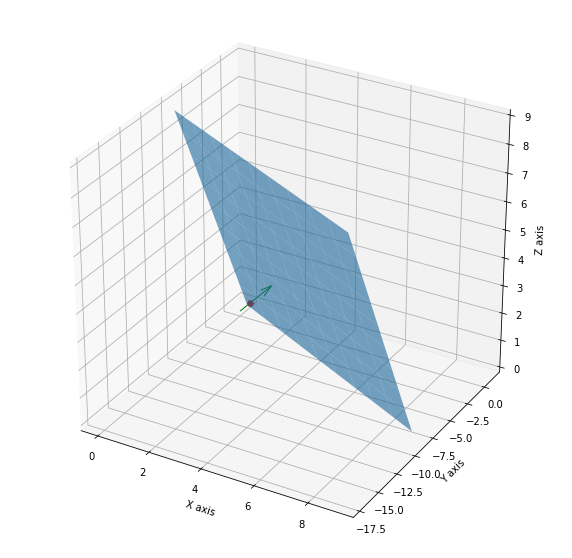
\includegraphics[width=\columnwidth]{plane3.png}
%    \caption{Perpendicular drawn from origin to the plane $\myvec{1&1&1}\vec{x} = 1$}
%    \label{myfig:solutions/line_plane/83}
%\end{figure}
%\ref{myfig:solutions/line_plane/83}
%\renewcommand{\thefigure}{b}
%\begin{figure}[h!]
%    \centering
%    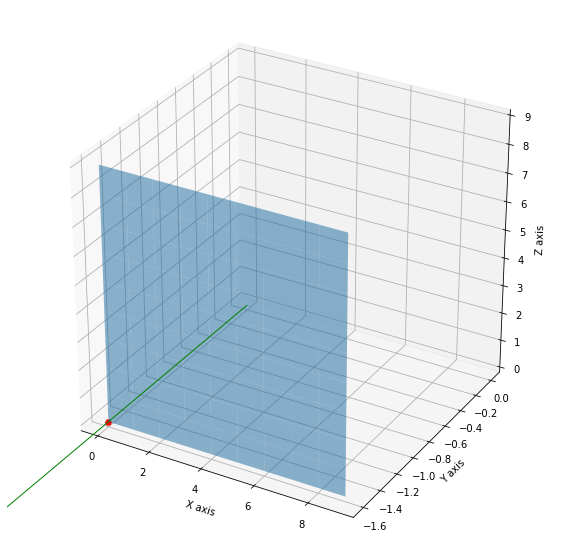
\includegraphics[width=\columnwidth]{plane4.png}
%    \caption{Perpendicular drawn from origin to the plane $\myvec{0&5&0}\vec{x} = -8$}
%    \label{myfig:solutions/line_plane/83}
%\end{figure}
